% !TeX root = ../OSN.tex

\subsection{Triadic Status}

Imagine there are two nodes named $A$ and $B$, and they are unlinked. What we want to do is to predict the weight of the edge from $A$ to $B$. Suppose that there is another node $X$, and $(A, B, X)$ compose a triangle once $A$ and $B$ are linked. Overall, there are four different triangle-links, as the edge between $X$ and $A$ can go in either direction and similarly for the edge between $X$ and $B$, if the sign of weight is not considered.

\begin{figure}[htbp]
\centering
	\begin{subfigure}{0.2\textwidth}
		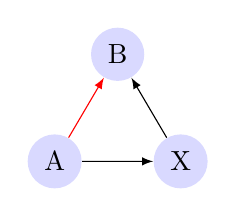
\begin{tikzpicture}
		[scale=0.8,every node/.style={circle,fill=blue!15}]
		  \node (A) at (1,1) {A};
		  \node (B) at (2,2.7)  {B};
		  \node (X) at (3,1)  {X};
		  \draw[->, >=latex, red] (A) edge (B);
		  \draw[->, >=latex] (A) edge (X);
		  \draw[->, >=latex] (X) edge (B);
		\end{tikzpicture}
		\caption{t1}
		\label{t1}
	\end{subfigure}
	\begin{subfigure}{0.2\textwidth}

		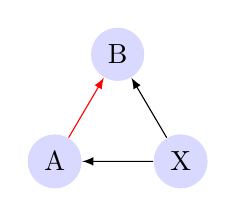
\begin{tikzpicture}
		[scale=0.8,every node/.style={circle,fill=blue!15}]
		\node (A) at (1,1) {A};
		\node (B) at (2,2.7)  {B};
		\node (X) at (3,1)  {X};
		\draw[->, >=latex, red] (A) edge (B);
		\draw[->, >=latex] (X) edge (A);
		\draw[->, >=latex] (X) edge (B);
		\end{tikzpicture}
		\caption{t2}
		\label{t2}
	\end{subfigure}
	\begin{subfigure}{0.2\textwidth}

		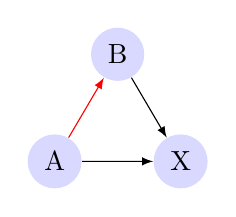
\begin{tikzpicture}
		[scale=0.8,every node/.style={circle,fill=blue!15}]
		\node (A) at (1,1) {A};
		\node (B) at (2,2.7)  {B};
		\node (X) at (3,1)  {X};
		\draw[->, >=latex, red] (A) edge (B);
		\draw[->, >=latex] (A) edge (X);
		\draw[->, >=latex] (B) edge (X);
		\end{tikzpicture}
		\caption{t3}
		\label{t3}
	\end{subfigure}
	\begin{subfigure}{0.2\textwidth}

		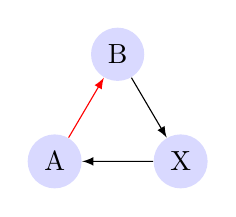
\begin{tikzpicture}
		[scale=0.8,every node/.style={circle,fill=blue!15}]
		  \node (A) at (1,1) {A};
		  \node (B) at (2,2.7)  {B};
		  \node (X) at (3,1)  {X};
		  \draw[->, >=latex, red] (A) edge (B);
		  \draw[->, >=latex] (X) edge (A);
		  \draw[->, >=latex] (B) edge (X);
		\end{tikzpicture}
		\caption{t4}
		\label{t4}
	\end{subfigure}
	\caption{Triadic Status}
	\label{Triadic Status Figure}
\end{figure}

And we predict the weight of the edge $(A, B)$ using three rules:

\begin{enumerate}

\item In Graph t1, the predicted weight of the transitive edge is the sum of the two non-transitive edge weights.

\item In Graph t2 and t3, the predicted weight of a non-transitive edge is the difference between the transitive and the other non-transitive edge weights. 

\item In Graph t4, since it is a cyclic triad, the weight of the missing edge is the negative of the sum of the other two edge weights.

\end{enumerate}

In the end, we take the average of predicted weights over all triadic-links that these two nodes are a part of.



